%!TEX root = ../notas_de_clase.tex

\section{Clasificación}

El problema de clasificación dice relación con la identificación del conjunto, categoría o \emph{clase} a la cual pertenece un elemento en base a sus \emph{características}. En el contexto del aprendizaje supervisado, el problema de clasificación puede ser visto como un caso particular del problema de regresión, donde el espacio donde la variable  $y$ (salida o variable dependiente) es \emph{categórico} y usualmente denotado por $\{0,1\}$, para el caso binario, o bien $\{1,2,\ldots,M\}$ para el caso de clasificación multiclase. 
	

\subsection{Formulación: clasificación lineal}
\label{sec:clasif_lineal}

\noindent\begin{minipage}{0.52\textwidth}
	Consideremos un conjunto de datos
	\begin{equation}
	 	\datos = \{(x_i,c_i)\}_{i=1}^N\subset\R^M\times\{\cC_i\}_{i=1}^K,
	 \end{equation}
	 donde, al igual que en el problema de regresión, $x$ es la variable independiente y $c$ es la variable dependiente o \emph{clase}. Consideraremos en primera instancia el caso \emph{binario}, es decir, solo dos clases ($K=2$), ilustrado en la Fig.~\ref{fig:puntos_2d}. Proponemos un modelo lineal para relacionar la variable independiente con su clase, es decir, 
	\begin{equation}
		y(x) = a^\top  x + b,
		\label{eq:clasificacion_lineal}
	\end{equation}
	donde la  asignación de la clase es de la siguiente forma: $x$ será asignado a $\cC_1$ si $y(x) \geq 0$ y será asignado $\cC_2$ en caso contrario.
\end{minipage}\hfill
%[AGREGAR IMAGEN]
\begin{minipage}{0.46\textwidth}
	\centering
	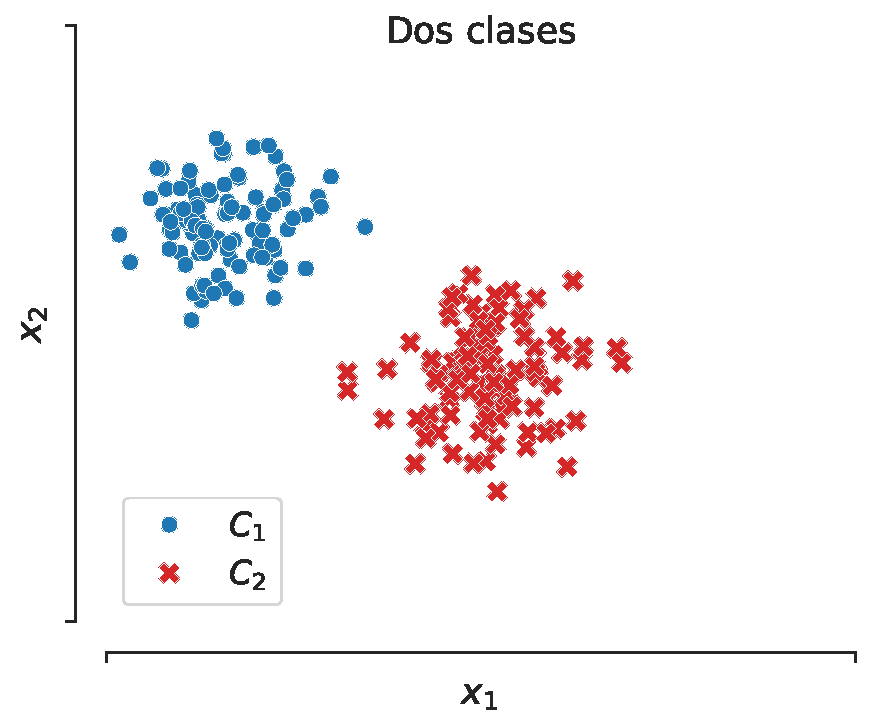
\includegraphics[width=\textwidth]{img/cap2_dosclases}\\
	\captionof{figure}{Ejemplo del problema  de clasificación binaria, donde la clase $\cC_1$ está presentada en azul y la clase $\cC_2$ en rojo.}
	\label{fig:puntos_2d}
\end{minipage}

\vspace{1cm}
Nos referiremos al subconjunto que particiona $\R^M$ en clase $\cC_1$ y clase $\cC_1$ como \emph{superficie/hiperplano/región de decisión}, la cual está definida por $y(x)=0$. Entonces, como $x\in\R^M$, para la consideración del modelo lineal esta superficie de decisión corresponde a un hiperplano de dimensión $M-1$.

Para resolver el problema de clasificación, debemos encontrar los parámetros $a$ y $b$ en la ec.~\eqref{eq:clasificacion_lineal}. Para este fin, veamos que si $x_1,x_2$ son dos puntos en la superficie de decisión, entonces tenemos la siguiente relación para el parámetro $a$:
\begin{align}
	0 &= y(x_1) - y(x_2) \nonumber\\
	  &= a^\top x_1 + b - a^\top x_2 - b \nonumber\\
	  &= a^\top (x_1-x_2).
\end{align}
Es decir, $a$ es ortogonal a cualquier vector que esté contenido dentro de la región de decisión. Intuitivamente, podemos decir que el vector $a\in\R^M$ controla la pendiente (u orientación) del hiperplano de decisión. Además, observemos que para cualquier $x$ en la región de decisión, i.e., $y(x)=0$,  su proyección en el vector $a$ está dada por  
\begin{equation}
	\frac{a^\top x}{\left \| a \right \|} = -\frac{b}{\left \| a \right \|},
\end{equation}
de donde podemos entender que el parámetro $b$ controla el desplazamiento (o ubicación) de la región de decisión,  pues el lado derecho de la ecuación representa la distancia entre la región de decisión y el origen.

Es posible  también interpretar $y(x)$ como una distancia con signo entre un $x\in\R^M$ cualquiera  y la superficie de decisión. Para ver esto, consideremos $x\in\R^M$ y descompongámoslo dos componentes: la primera denotada por $x_{\bot}$, la cual es la proyección ortogonal de $x$ en el hiperplano de  decisión, y la segunda que es perpendicular al hiperplano (y consecuentemente paralela al vector $a$) denotada por $r\frac{a}{\left \| a \right \|}$, donde $r$ denota la distancia entre $x$ y el  hiperplano de  decisión. Expresamos entonces  
\begin{equation}
	x = x_{\bot}+r\frac{a}{\left \| a \right \|},
\end{equation}
y observamos que
\begin{equation}
	y(x) 
	= a^\top x+b 
	=a^\top  \left( x_{\bot} + r\frac{a}{\left \| a \right \|} \right) +b 
	= \underbrace{a^\top x_{\bot} +b }_{=0} +   r\frac{a^\top  a}{\left \| a \right \|}
	= r||a||.
\end{equation}
Consecuentemente, vemos que $\forall x\in\R^M$, $r = \frac{y(x)}{||a||}$,  es decir, $y(x)$ representa una medida con signo de la  distancia entre el punto $x$ y la  región de decisión. 

El caso de múltiples clases ($K>2$) puede ser enfrentado mediante una extensión del caso binario. Una forma puede ser construir $K-1$ clasificadores binarios, en donde cada uno  resuelve el problema de discriminar los elementos de la  clase $\cC_k$ del resto; esta técnica se llama \emph{one-versus-rest}. Otra forma es construir $K(K-1)/2$ clasificadores binarios, donde cada uno discrimina entre cada posible par de clases; esta técnica se llama \emph{one-versus-one}. El problema con estas dos alternativas es que dejan  regiones indefinidas en el espacio, pues solo consideran pares de clases que  al ser agregados pueden ser incoherentes. 

Una alternativa más robusta para resolver el problema de clasificación multiclase es construir un clasificador para $K$ clases que contiene $K$ funciones lineales de la forma
\begin{equation}
	y_k(x) = a_k^\top x + b_k, \quad k=1,\ldots,K.
\end{equation}
Donde $x$ es asignado a la clase $\mathcal{C}_k$ si y solo si $y_k(x) > y_j(x), \forall j\neq k$, es decir:

\begin{equation}
	\mathcal{C}(x) = \underset{k}{\argmax}\hspace{1mm} y_j(x).
\end{equation}

La región de decisión de este clasificador de $K$ clases es efectivamente convexa y no  quedan secciones de $\R^M$ sin asignar clase (o con asignación incoherente). Además, si elegimos $K=2$, obtenemos el clasificador  binario. (Esto puede quedar de tarea 3)

\subsection{Ajuste mediante mínimos cuadrados}

Ya hemos planteado el modelo y analizado el rol  y significado de cada uno de sus parámetros; ahora queda por estudiar cómo determinar dichos parámetros $a$ y $b$, dado un conjunto de datos $\datos$. Para esto consideraremos en primer lugar el enfoque de mínimos cuadrados, el cual es la medida de discrepancia  por  excelencia  y a primera vista  parece una respuesta natural a este problema. Primero  introduciremos un poco de notación para plantear el problema de forma clara.

Consideremos el  punto $x\in\R^M$ con clase $c\in\{\mathcal{C}_k\}_{k=1}^K$. Usaremos la \emph{codificación} $t \in\{0,1\}^K$ para representar la pertenencia de $x$ a su respectiva clase. Es decir, 
\begin{equation}
	c = \cC_j \Leftrightarrow [t]_j=1 \wedge [t]_i=0, \quad i\neq j.
\end{equation}
Este tipo de codificación  es conocida como \emph{one-hot  encoding.}  

\begin{remark}
Usamos esta codificación por  dos razones. Primero, para poder dar valores numéricos a la clase y que  podamos hablar de distancias entre ellos, pues si nuestras clases son ``peras y manzanas'' necesitamos poder determinar cuán cerca a cada una de ellas está nuestra estimación. En segundo  lugar, como los valores asignados al vector $t$ siempre serán puros 0's y un solo 1, entonces  todos los posibles  valores de $t$ están a la misma distancia unos de otros. De esta forma, si dos elementos tienen distintas clases, la distancia entre éstas, cualquieras sean, será 0 (clases iguales), o bien $\sqrt{2}$ (clases distintas). Esto ayuda a no introduce sesgos en la representación de la clase que puedan alterar el aprendizaje del modelo.  	
\end{remark}

Asumiendo entonces el modelo lineal para cada clase $\mathcal{C}_k$ dado por
\begin{equation}
	y_k(x) = a_k^\top x + b_k,
\end{equation}
podemos reescribir el modelo de forma matricial como:	
\begin{equation}
	y(x) = \tilde{\Theta}^\top \tilde{x}.
\end{equation}
Donde la $k$-esima columna de $\tilde{\Theta}$ es un vector de $M+1$ dimensiones definido por $\tilde{\theta}_k=[b_k, a_k^\top]^\top$, $\tilde{x}=[1,x^\top]^\top$ corresponde al vector $x$ aumentado y la cantidad $y(x)$ es el vector de \emph{asignaciones de clases}. De esta forma, un punto $x$ será asignado a la clase que tenga mayor $y_k=\tilde{\theta}_k^\top \tilde{x}$. Es  decir, la clase de $x$ es modelada como  el  $\argmax y(x)$.

Con la notación establecida, ahora podemos enfocarnos en el entrenamiento del modelo. Para esto consideremos un conjunto de entrenamiento $\{(x_n,t_n)\}_{n=1}^N$, y definamos las siguientes matrices:
\begin{align}
	T &= [t_1, t_2,\ldots, t_N]^\top\\
	\tilde{X} &= [\tilde{x}_1, \tilde{x}_2, \ldots, \tilde{x}_N ]^\top.
\end{align}
Con lo que estamos en posición de determinar los coeficientes de $\tilde{\Theta}$ mediante la minimización de la suma de los errores cuadráticos de forma similar al problema de regresión. Podemos escribir la función de costovde la siguiente forma:
\begin{equation}
	J(\tilde{\Theta}) = \trace{(\tilde{\Theta}\tilde{X}-T)^\top(\tilde{\Theta}\tilde{X}-T)},\label{eq:K-class-LS}
\end{equation}
donde $\trace{\cdot}$ corresponde al operador traza. Al aplicar la condición de primer orden a la ec.~\eqref{eq:K-class-LS} (i.e., derivar e igualar a 0), obtenemos la solución de mínimos cuadrados para el problema de clasificación dado por:
\begin{equation}
	\tilde{\Theta} = (\tilde{X}^\top\tilde{X})^{-1}\tilde{X}T,
\end{equation}
con lo que la predicción de la clase para un nuevo input $x$ está dada por $ y(x) = T^\top\tilde{X}^\top(\tilde{X}^\top\tilde{X})^{-1}\tilde{x}$.

\begin{remark} Hay dos problemáticas conceptuales con este enfoque. En primer lugar, el uso de mínimos cuadrados es muy sensible a la presencia de puntos aislados (\emph{outliers}). Dado el crecimiento cuadrático de la penalización, los puntos lejanos al promedio de los datos tienen una influencia mucho mayor. Esto ciertamente afecta considerablemente los resultados y no es coherente con el problema de clasificación, donde la estimación es correcta o incorrecta, pero no ``más'' o ``menos'' correcta. Este efecto sobre la solución es ilustrado en la Figura \ref{fig:clasif_mse}, en donde la presencia de puntos alejados de clase $\cC_2$ afecta el resultado (derecha), incluso donde el resultado original (izquierda) estaba correcto. En segundo lugar, las predicciones de  clase  $y(x)$ no tienen la forma de las etiquetas originales $t$, con lo cual es necesario una intervención ``manual'' en donde, dado un $y(x)$ debemos definir el $t(x)$ apropiado. 
\end{remark}


\begin{figure}[H]
	\centering
	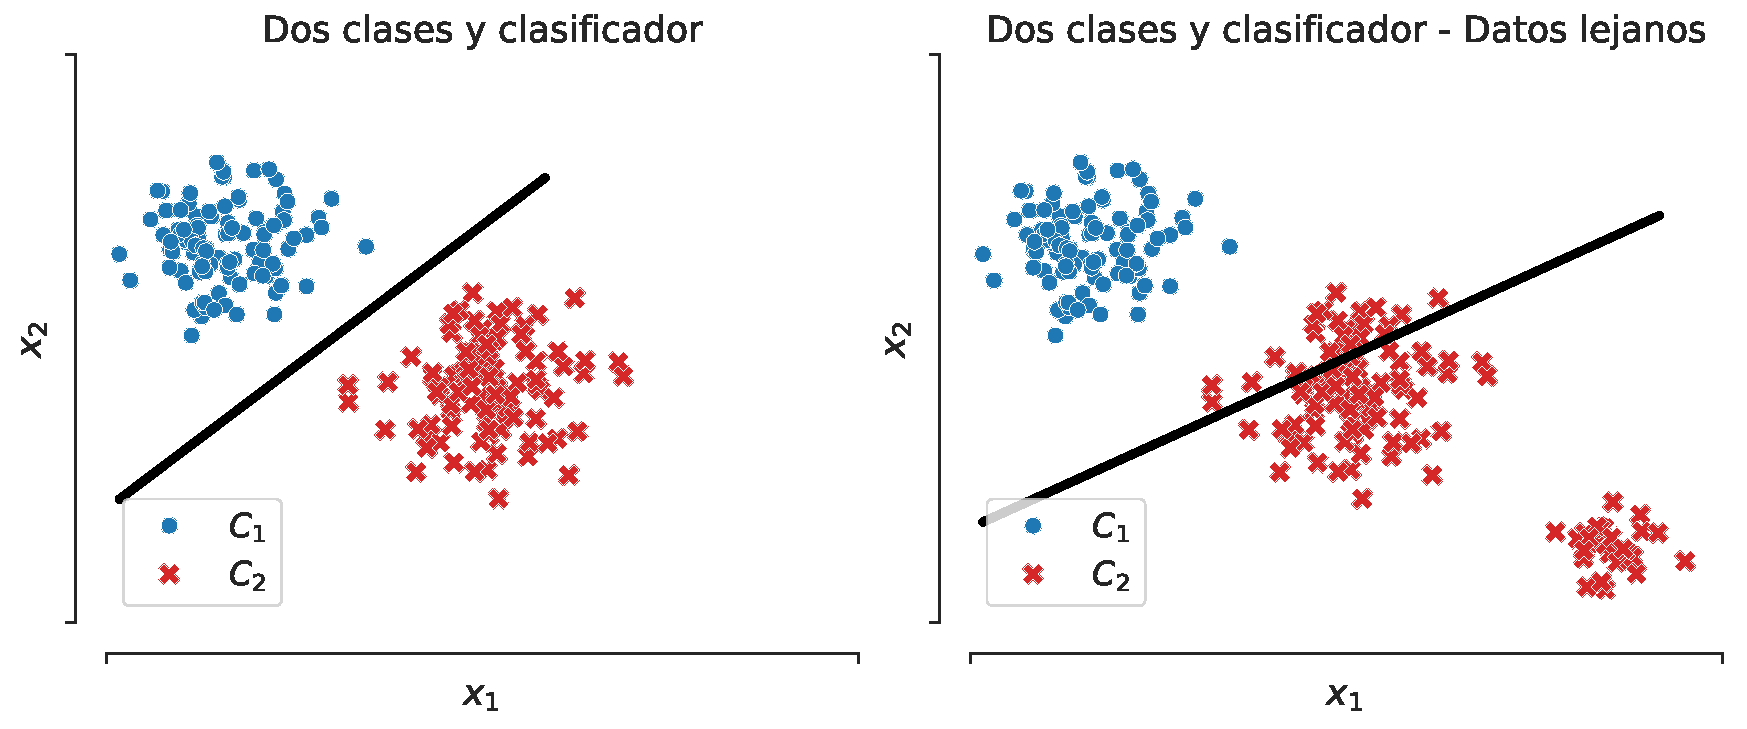
\includegraphics[width=0.8\textwidth]{img/cap2_dosclases_clasificador.pdf}\\
	\caption{Ejemplo ilustrativo sobre cómo los puntos lejanos de una clase pueden afectar incorrectamente los resultados.}
	\label{fig:clasif_mse}
\end{figure}

\subsection{Discriminante lineal de Fisher}

Para evitar los artefactos (sesgos) introducidos por clases  asimétricas en el uso de mínimos cuadrados para clasificación, es posible interpretar el problema de clasificación como uno de \emph{reducción de dimensionalidad}\footnote{El problema de reducción de dimensionalidad consiste con construir una representación de dimensión estrictamente menor que los datos originales con la finalidad de interpretar de mejor forma la información contenida en nuestros datos}, en donde la reducción consiste representar nuestros datos  en solo una dimensión, la cual representa su (grado de pertenencia a una) clase. Con este objetivo en mente, consideremos el problema de clasificación binaria y $x\in R^D$ para proyectos $x$ en un espacio unidimensional de la  siguiente forma:
\begin{equation}
	y = a^\top x,
\end{equation}
donde podemos definir un umbral $b$ para asignar $x$ a $\cC_1$ si $y\geq-b$ y $x$ a $\cC_2$ en caso contrario. Notemos que de esta forma recuperamos el modelo lineal para clasificación presentado al comienzo de este capítulo.

En general, al proyectar el objeto $D$-dimensional en un espacio  1-dimensional, se pierde gran cantidad de la información, lo cual expresa en el hecho que clases claramente separadas en el espacio $D$-dimensional pueden traslaparse al ser proyectadas a 1 dimensión cuando la elección del vector $a$ no es la correcta. Sin embargo, es posible ajustar el vector $a$ tal que se  garantice que una proyección en éste maximice el grado de separación entre clases.

Para encontrar el $a$ que cumple con este requerimiento en base a un conjunto de datos  $\datos$, definamos las cardinalidades de clases mediante $N_1 = |\{x|x\in\cC_1\}|$ y $N_2 = |\{x|x\in\cC_2\}|$, lo cual permite calcular los promedios (muestrales) de cada  clase mediante: 
\begin{equation}
	\mu_1=\frac{1}{N_1}\sum_{n\in\mathcal{C}_1}x_n
	\quad\quad\quad
	\mu_2=\frac{1}{N_2}\sum_{n\in\mathcal{C}_2}x_n.
\end{equation}
La medida más simple de separación entre las proyecciones de las clases sobre $a$ es la distancia entre las medias  de sus proyecciones.
\begin{equation}
	m_1 - m_2 = a^\top(\mu_1-\mu_2),
\end{equation}
donde $m_k= a^\top\mu_k$ corresponde al promedio de los elementos de  la clase $\mathcal{C}_k$ proyectado sobre el  vector $a$. Consecuentemente, el vector $a$ que maximiza la distancia entre la proyección de clases es el que maximiza la expresión anterior. Sin embargo, esta expresión puede ser arbitrariamente grande si escalamos $a$, entonces, para evitar estas redundancias impondremos que $\left \| a \right \|_2=1$. Usando multiplicadores de Lagrange para optimizar el problema restringido se llega a que $a\propto(\mu_1-\mu_2)$. 

Una desventaja de este enfoque, en el cual se ha ignorado la dispersión de las clases y solo se ha considerado su media, es que pueden existir 2 clases bien separadas en el espacio $D$-dimensional, pero al proyectar los datos sobre la recta que une sus promedios, las proyecciones de cada clase se traslapen. Para resolver este problema, Fisher propuso maximizar más que la mera distancia entre las (medias de las) clases proyectadas, sino que adicionalmente minimizar la dispersión de las  muestras de una misma clase con el objetivo de disminuir el traslape entre las proyecciones de las clases. 

Como medida de dispersión, definimos la varianza de los elementos de la clase $\cC_k$ mediante
\begin{align}
	s_k^2 &= \sum_{n\in \mathcal{C}_k}(a^\top(x_n-\text{m}_k))^2\\
	&= \sum_{n\in \mathcal{C}_k}(y_n-m_k)^2,
\end{align}
lo cual nos permite definir la siguiente función objetivo
\begin{equation}
J(a) = \frac{m_1-m_2}{s_1^2+s_2 ^2},
\end{equation}
donde explícitamente vemos la discrepancia ``inter'' clases en el numerador y la discrepancia  ``intra '' clases en el numerador. Adicionalmente, podemos expresar este costo directamente como función de el vector de proyección $a$:
\begin{equation}
	J(a) = \frac{a^\top S_B a}{a^\top S_Wa}.
\end{equation}
Donde la matriz de covarianza entre clases $S_B$ y matriz total de covarianza dentro de clases $S_W$ están respectivamente dadas por
\begin{align}
	S_B &= (\mu_1-\mu_2)(\mu_1-\mu_2)^\top\\
	S_W &= \sum_{n\in \cC_1}(x_n-\mu_1)(x_n-\mu_1)^\top +
	\sum_{n\in \cC_2}(x_n-\mu_2)(x_n-\mu_2)^\top. 
\end{align}
Aplicando la condición de primer orden para $J(a)$, obtenemos que el vector $a$ óptimo debe cumplir
\begin{equation}
	(a^\top S_B a)S_W a = (a^\top S_W a)S_B a.	
\end{equation}
Sin embargo, notemos que la norma del vector  $a$ es irrelevante, solo interesa su orientación, con lo que  ignorando los escalares $(a^\top S_B a)$ y $(a^\top S_W a)$ tenemos que la relación de optimalidad es $S_W a \propto S_B a$. Además, por la definición de $S_B$, sabemos que $S_B a\propto(\mu_1-\mu_2)$, con lo que la relación de optimalidad se convierte en es $S_W a \propto (\mu_1-\mu_2)$. Consecuentemente, el vector $a$ que cumple el  criterio de Fisher es 
\begin{equation}
	a \propto S_W^{-1}(\mu_1-\mu_2).
\end{equation}

La Figura \ref{fig:ej_fda} muestra el  discriminador lineal que solo considera los promedios a la  izquierda y la corrección de Fisher a la derecha. Observemos cómo el incluir una medida de la dispersión de los datos es clave para lograr un mejor discriminador.

\begin{figure}[H]
	\centering
	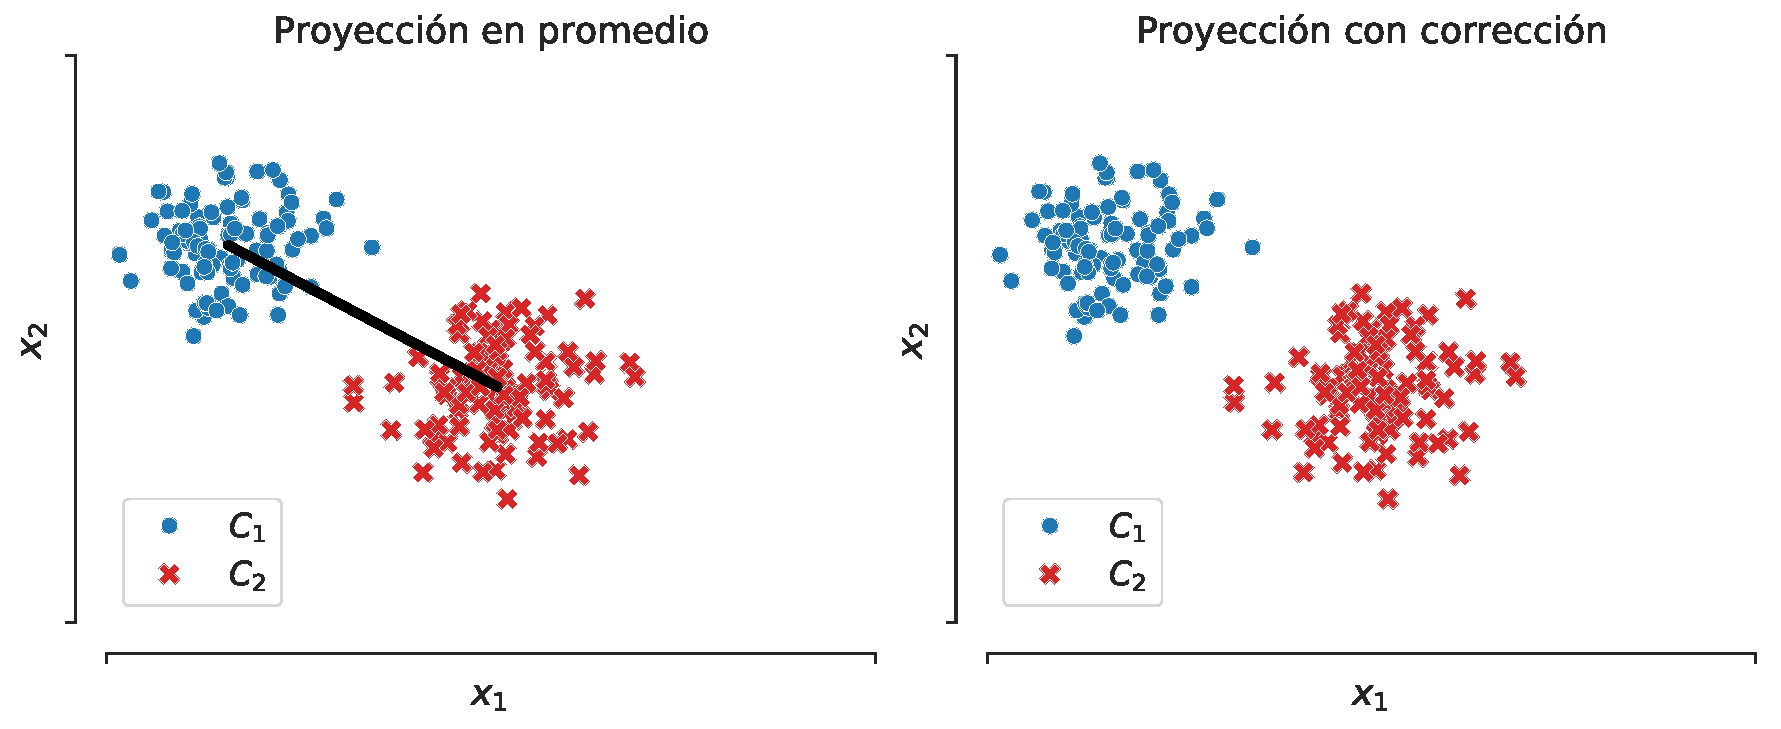
\includegraphics[width=0.8\textwidth]{img/cap2_dos_clases_proyeccion.pdf}
	\caption{Discriminador lineal considerando solo la media entre clases (izquierda) y  su extensión mediante la corrección de Fisher que incorpora la varianza muestral de los datos.}
	\label{fig:ej_fda}
\end{figure}


\subsection{Clasificación No Lineal: El Perceptrón}

Las nociones básicas que hemos visto hasta ahora para lidiar con el problema de clasificación tiene dos problemáticas conceptuales. La primera es la falta de una métrica correcta para evaluar la bondad de nuestro modelo,  esto es porque el criterios de mínimos cuadrados no es apropiado en la evaluación de una asignación de clases, donde no hay concepto de ``más cerca'', sino que solo correcto/incorrecto. Además, todos los enfoques considerados en esta sección hasta este punto no tienen una \emph{función de versoimilitud} apropiada que conecte el modelo (variables latentes) con la clase  (observación) de forma coherente. Por el contrario, hasta ahora hemos considerado que  por un lado está el modelo lineal para clasificación y por otro lado está \emph{nuestra decisión} de la clase en base a la salida del modelo linear, por  ejemplo si $y(x)>b$ decimos que ``$x$ es clase $\cC_1$''.

Como veremos a continuación, ambas problemáticas se resuelven de forma simultánea, pues mediante el diseño de una función de verosimlitud resolvemos la damos la capacidad al modelo de entregar directamente la clase como  output y en base a esta  verosimilitud se define  una función de costo. Sin embargo, el desafío más importante en esta construcción es que el modelo resultante ya no es lineal, ni en la entrada ni en los parámetros, pues una verosimilitud lineal nunca nos  llevará de un espacio de inputs (hemos asumido $\R^M$) al espacio de categorías $\{\cC_1,\cC_2,\ldots,\cC_k\}$.

Una forma de resolver estas problemáticas es mediante el uso del \emph{Perceptrón} \cite{rosenblatt_1958}, un modelo de clasificación binario que tuvo mucha importancia en el área de reconocimiento de patrones. El Perceptrón consiste en una función no-lineal fija usada para transformar $x$ en un vector de características $\phi(x)\in\R^D$, que luego es usado para generar un modelo lineal \emph{generalizado} es decir, un modelo lineal concatenado con una función no lineal $f(\cdot)$ de la siguiente forma:
\begin{align}
	y(x) &= f(\theta^\top\phi(x))\\
	f(u) &= \left\{\begin{matrix}
	+1,\quad u\geq 0\\
	-1,\quad u<0
	\end{matrix}\right.
\end{align}
Donde opciones típicas para el vector $\phi(x)$ es concatenar la entrada con un intercepto para la recta, es decir $\phi(x) = [x^\top, 1]$ como vimos al comienzo del curso, o bien características no lineales como las vistas en la Sección \ref{sec:reg_no_lineal}. El Perceptrón entonces asigna $x$ a la clase $\mathcal{C}_1$ si $y(x)=+1$ y asignará $x$ a la clase $\mathcal{C}_2$ cuando $y(x)=-1$. Notemos que  para  el caso que $\phi$ es lineal, este es el mismo clasificador presentado en la Sección \ref{sec:clasif_lineal}, pero en este caso el criterio para asignar la clase es \textbf{parte del modelo}.

Una condición para determinar el parámetro $\theta\in\R^D$ en base a un conjunto de datos  $\datos = \{(x_i,t_i)\}_{i=1}^N$, es que para $x\in\mathcal{C}_1$ ($t=1$), se cumpla que $\theta^\top\phi(x) > 0$, y para $x\in\mathcal{C}_2$ ($t=-1$) se cumpla $\theta^\top \phi(x) < 0$. Usando el hecho que las etiquetas están representadas por la  codificación $t\in\{1,-1\}$, ambas condiciones pueden ser cubiertas por la expresión:
\begin{equation}
	\theta^\top\phi(x_n)t_n > 0,\quad \forall (x_n,t_n) \in \datos.
\end{equation}

Podemos entonces satisfacer esta restricción mediante el ``criterio del perceptrón'', el cual se basa en los elementos de $\datos$ que fueron clasificados incorrectamente. Este criterio asocia a los puntos clasificados correctamente 0 error y a los puntos mal clasificados error $-\theta^\top\phi(x)t$, de esta forma que si denotamos como $\mathcal{M}$ el conjunto de puntos mal clasificados, se debe minimizar la siguiente función objetivo:
\begin{equation}
	J_\text{P}(\theta) = -\sum_{i\in\mathcal{M}}\theta^\top\phi(x_i)t_i. 
\end{equation}
Observemos que al no usar directamente la función de activación perceptrón $f(\cdot)$, este costo es diferenciable (asumimos que $\phi(\cdot)$ lo es), con lo que podemos  minimizarla mediante \emph{descenso de gradiente estocástico}. Para cada elemento $x_i\in\mathcal{M}$, estas actualizaciones toman la siguiente forma:
\begin{align}
	\theta^{\tau+1} &= \theta^\tau - \eta \nabla J_\text{P}(\theta)\\
	&= \theta^\tau + \eta \phi(x_i)t_i.\label{eq:percetron_rule}
\end{align}
La variable $\tau\in\N$ simplemente indexa la secuencia $\{\theta_0,\theta_1,\ldots\}$, la cual  parte de un $\theta_0$ arbitrario y esperamos que converja al parámetro apropiado. El hyperparámetro $\eta$ es una constante que se conoce como \emph{tasa de aprendizaje}. Sin embargo, como la función perceptrón $y(x)=y(x,\theta)$ no cambia si $\theta$ se amplifica por una constante arbitraria; entonces, sin perdida de generalidad, podemos asumir que $\eta=1$. Es importante notar que al actualizar el vector $\theta$, el conjunto de puntos mal clasificados $\mathcal{M}$ va a cambiar, pues (esperamos que) en vada iteración los elementos del conjunto de puntos mal clasificados vaya disminuyendo.

La interpretación del algoritmo usado para ajustar el perceptrón es simple, debido al uso del gradiente estocástico, se recorre el conjunto de puntos de entrenamiento $\{x_n\}_{n=1}^N$, si el punto $x_n$ fue clasificado correctamente el vector de pesos de mantiene igual. Sin embargo, $x_n$ fue clasificado incorrectamente, el vector $\theta^\tau$ es actualizado según la ec.~\eqref{eq:percetron_rule} con $\eta=1$ mediante
\begin{equation}
	 \theta^{\tau+1} = \theta^\tau + \phi(x_i)t_i,
\end{equation}
es decir, el parámetro $\theta$ está paso a paso modificado en la dirección de las características $\phi(x_i)$ con multiplicador $\pm1$ en base a la clase verdadera de $x_i$ hasta  que todos los puntos de $\datos$ están bien clasificados. 

\subsection{Clasificación Probabilista}

Los modelos que hemos revisado hasta este punto son del tipo \emph{discriminativo}, es decir, modelan directamente la función $f:x\mapsto c$, o  en el caso probablístico, la probabilidad condicional $\mathbb{P}(\mathcal{C}_k|x)$, es decir, dado que conozco el input o características $x$, cuál es la distribución de probabilidad sobre las clases. En particular, hemos considerado métodos determinísticos, que  solo asignan pobabilidad 1 a una sola clase. Otro paradigma más poderoso a considerar es un enfoque generativo en el cual modelamos dos  objetos: en primer lugar la ``probabilidad condicional de clase'' la cual modela cómo distribuyen los valores de los inputs $x$ cuando la  clase es, por  ejemplo $\cC_k$, denotada por $\mathbb{P}(x|\mathcal{C}_k)$. En segundo lugar las ``probabilidades de clase'', o el prior sobre clases, denotada $\mathbb{P}(\mathcal{C}_k)$. Luego, podemos calcular la densidad posterior sobre las clases dado un input $x$ usando el Teorema de Bayes de acuerdo a 
\begin{equation}
	\mathbb{P}(\mathcal{C}_k|x) = \frac{\mathbb{P}(x|\mathcal{C}_k)\mathbb{P}(\mathcal{C}_k)}{\mathbb{P}(x)}.
\end{equation}

Ilustremos la forma de esta distribución en primer lugar para el caso de 2 clases. Podemos calcular la probabilidad de la clase $\cC_1$ dado $x$ de la forma:
\begin{align}
	\mathbb{P}(\mathcal{C}_1|x) &= \frac{\mathbb{P}(x|\mathcal{C}_1)\mathbb{P}(\mathcal{C}_1)}{\mathbb{P}(x)}\nonumber\\
	&= \frac{\mathbb{P}(x|\mathcal{C}_1)\mathbb{P}(\mathcal{C}_1)}{\mathbb{P}(x|\mathcal{C}_2)\mathbb{P}(\mathcal{C}_2)+\mathbb{P}(x|\mathcal{C}_1)\mathbb{P}(\mathcal{C}_1)}\nonumber\\
	&=\frac{1}{1+\frac{\mathbb{P}(x|\mathcal{C}_1)\mathbb{P}(\mathcal{C}_1)}{\mathbb{P}(x|\mathcal{C}_2)\mathbb{P}(\mathcal{C}_2)}}\nonumber\\
	&=\frac{1}{1+\exp(-r)} = \sigma(r).\label{eq:logistic1}
\end{align}

Donde hemos introducido la notación $r = r(x) =\ln\left(\frac{\mathbb{P}(x|\mathcal{C}_1)\mathbb{P}(\mathcal{C}_1)}{\mathbb{P}(x|\mathcal{C}_2)\mathbb{P}(\mathcal{C}_2)}\right)$  y la  función logística definida mediante $\sigma(r) = \frac{1}{1+e^{-r}}$, la cual  tiene propiedades que serán útiles en el entrenamiento, en particular, 
\begin{align}
	\text{reflejo: }\sigma(-r)&=1-\sigma(r)\\
	\text{derivada: }\frac{d}{dr}\sigma(r)&=\sigma(r)(1-\sigma(r))\\
	\text{inversa: }r(\sigma)&=\ln\left(\frac{\sigma}{1-\sigma}\right).
\end{align}


\begin{remark} Si bien la expresión de la distribución condicional en la ec.~\eqref{eq:logistic1} parece una presentación antojadiza para hacer aparecer la  función logística (sigmoide), pues $r=r(x)$ puede ser cualquier cosa, veremos que existe una elección particular de las distribuciones condicionales de clase que lleva a un $r$ que es efectivamente lineal en $x$. En general, nos  referiremos como \textbf{regresión logistica} en dicho caso,  cuando $r(x) = a^\top x  + b$.
\end{remark} 

Podemos ahora considerar el caso de múltiples clases $\{\cC_1,\ldots,\cC_K\}$, donde podemos hacer un desarrollo similar al anterior:  
\begin{equation}
	\mathbb{P}(\mathcal{C}_i | x) = \frac{\mathbb{P}(x | \mathcal{C}_i)\mathbb{P}(\mathcal{C}_i)}{\sum_{j}\mathbb{P}(x | \mathcal{C}_j)\mathbb{P}(\mathcal{C}_j)} = \frac{\exp(s_i)}{\sum_{j\neq i}\exp(s_j)}.\label{eq:softmax1}
\end{equation}
Donde hemos denotado $s_i = \mathbb{P}(x | \mathcal{C}_i)\mathbb{P}(\mathcal{C}_i)$. La función que aparece al lado derecho de la  ec.~\eqref{eq:softmax1} se conoce como \emph{exponencial inversa} o \emph{softmax} y corresponde a una generalización de la función logística a múltiples clases. Además,  tiene la propiedad de ser una aproximación suave de la función máximo y convertir cualquier vector $s=[s_1,\ldots,s_k]$ en una distribución de probabilidad, donde podemos hablar de ``la probabilidad de ser clase $\cC_k$''.

\subsubsection{Regresión logística} 
\label{sub:reg_log}

Analizaremos ahora  los supuestos sobre el modelo generativo (i.e., las  probabilidades de clase y condicionales) para encontrar un $r$---en la ec.~\eqref{eq:logistic1}---que resulta en la bien conocida regresión logística. Consideraremos el caso en donde las densidades condicionales de clase son Gaussianas multivariadas, dadas por
\begin{equation}
	p(x|\mathcal{C}_k) \sim \mathcal{N} (\mu_k,\Sigma) = \frac{1}{(2\pi)^\frac{D}{2}|\Sigma|^\frac{1}{2}}\exp(-\frac{1}{2}(x-\mu_k)^\top \Sigma^{-1}(x-\mu_k)).
\end{equation}
En cuyo caso obtenemos $r$ en ec.~\eqref{eq:logistic1}  dado por
\begin{align}
r &= \ln(\exp(-\frac{1}{2}(x-\mu_1)^\top \Sigma^{-1}(x-\mu_1) +\frac{1}{2}(x-\mu_2)^\top \Sigma^{-1}(x-\mu_2)))= \theta^\top x+w,
\end{align}
donde hemos usado la notación
\begin{align}
\theta &= \Sigma^{-1}(\mu_1-\mu_2)\\
w &= \frac{1}{2}(\mu_1^\top \Sigma^{-1}\mu_1+\mu_2^\top \Sigma^{-1}\mu_2)
+\ln\left(\frac{p(\mathcal{C}_1)}{p(\mathcal{C}_1)}\right). 
\end{align}
Lo cual nos entrega la regresión logística (lineal) para el  caso binario, donde al incorporar la expresión anterior en la ec.~\eqref{eq:logistic1} obtenemos
\begin{equation}
	p(\mathcal{C}_k|x) = \sigma(\theta^\top x+w) = \frac{1}{1 + \exp{\left(\theta^\top x+w\right)}}. \label{eq:logistica2}
\end{equation}

\begin{remark}\label{rem:reg_log} 
El modelo de clasificación binaria en la  ec.~\ref{eq:logistica2} es conocido como \emph{regresión logística} y es la consecuencia de asumir un modelo generativo Gaussiano con distintas medias pero la misma varianza para una de las clases. Como consecuencia, la región de decisión se encuentra imponiendo que la probabilidad de ser clase $\cC_1$ sea 1/2 (y por ende, ser $\cC_2$ también tiene probabilidad 1/2), lo cual se tiene para 
\begin{equation}
	\theta^\top x+w = 0.
\end{equation}
\end{remark}

Ahora que hemos definido el modelo para nuestro problema de clasificación, aflora naturalmente la siguiente pregunta: ¿Cómo ajustar los parámetros de las condicionales a la clase y priors respectivamente? Para esto, reiteremos que los parámetros del modelos serán los de la probabilidad de clase $(\pi)$ y de la probabilidades condicionales de clase. Respectivamente: 

\begin{itemize}
	\item Probabilidad de clase
	\begin{equation}
	 	p(\mathcal{C}_1)=\pi,\quad  p(\mathcal{C}_2)=1-\pi,\label{eq:prob_clase}
	 \end{equation}  es decir,  un parámetro $\pi$
	\item Probabilidad condicional de clase 
	\begin{equation}
		p(x|\mathcal{C}_k) = \mathcal{N}(\mu_k,  \Sigma); k=1,2,\label{eq:prob_clase_cond}
	\end{equation} 
	es decir, parámetros $ \mu_1\in\R^M,\mu_2\in\R^M,\Sigma\in\R^M\times\R^M$ o, equivalentemente, $M + M + M(M+1)/2=M(M+5)/2$ parámetros escalares. 
\end{itemize}
Los cuales denotaremos mediante el parámetro agregado $\theta =\{\mu_1,\mu_2,\Sigma \}$.

Realizaremos el entrenamiento del modelo, i.e., encontrar los parámetros descritos en las últimas expresiones en base a un conjunto de datos $\datos$, mediante el método de máxima verosimilitud. Para esto, notemos que solo hemos definido ``la probabilidad de ser clase $\cC_1$'', con lo que la verosimilitud de una observación $(x_i,t_i)$, con $t_i = 0$ si $x\in\cC_0$ y \emph{viceversa}, puede ser expresada mediante
\begin{equation}
	l_i(\theta) = p(x_i, t_i|\theta) =  p(x_i,\cC_1|\theta)^{t_i}p(x_i,\cC_0|\theta)^{1-t_i}, 
\end{equation}
ya que esta expresión equivale a la probabilidad de ser clase $\cC_1$ cuando $t_i=1$ y a la probabilidad de ser clase $\cC_0$ cuando $t_i=0$. Consecuentemente, para un conjunto de datos $\datos$ de la forma
	\begin{align}
	T&=(t_1,t_2,\ldots,t_N) \in \{0,1\}^N\\
	X&=(x_1,x_2,\ldots,x_N),
	\end{align}
podemos escribir la verosimilitud mediante $l(\theta) = p(X,T|\pi,\mu_1,\mu_2,\Sigma) $
\begin{align}
	l(\theta) &= \prod_{i=1}^{N}p(x_i,t_i|\pi,\mu_1,\mu_2,\Sigma)\nonumber\\
	&= \prod_{i=1}^{N}p(x_i,\mathcal{C}_1)^{t_i}p(x_i,\mathcal{C}_0)^{1-t_i}\nonumber\\
	&= \prod_{i=1}^{N}(\pi\mathcal{N}(x_i|\mu_1,\Sigma))^{t_i}
	((1-\pi)\mathcal{N}(x_i|\mu_2,\Sigma))^{1-t_i}.
	\end{align}

AL igual que en el escenario de regresión lineal, para proceder con la optimización nos enfocamos en la log-verosimilitud, dada por:	
	\begin{equation}
	\log(L) := \sum_{i=1}^{N}t_i(\log(\pi)+\log(\mathcal{N}(x_i|\mu_1,\Sigma)))+(1-t_i)(\log(1-\pi)+\log(\mathcal{N}(x_i|\mu_2,\Sigma))). 
		\end{equation}

Aplicando entonces las condiciones de primer orden, tenemos que 
\begin{itemize}
	
\item \textbf{1)}Con respecto a $\pi$:
	
	\begin{align}
	\frac{\partial\log(L)}{\partial\pi} &= \sum_{i=1}^N \frac{t_i}{\pi}+\frac{1-t_i}{1-\pi}=0\nonumber\\
	\Rightarrow \quad & (i-\pi)\sum_{i=1}^Nt_i = \pi\sum_{i=1}^N(1-t_i)\nonumber\\
	\Rightarrow \quad & \sum_{i=1}^Nt_i=\pi N \quad\Rightarrow\quad \pi = \frac{\sum_{i=1}^Nt_i}{N} = \frac{N_1}{N_1+N_2} \label{eq:log_reg_pi}
	\end{align}
		
\item \textbf{2)}Con respecto a $\mu_1$:
	
	\begin{align}
	\frac{\partial\log(L)}{\partial\mu_1} &= \sum_{i=1}^N t_i
	\frac{\partial}{\partial \mu_1}(-\frac{1}{2}(x_i-\mu_1)^\top \Sigma^{-1}(x_i-\mu_1))\nonumber\\
	&= \sum_{i=1}^N t_i(\Sigma^{-1}(x_i-\mu_1)) =
	\Sigma^{-1}\sum_{i=1}^N t_i(x_i-\mu_1) = 0\nonumber\\
	\Rightarrow\quad & \sum_{i=1}^Nt_ix_i= \mu_1\sum_{i=1}^N t_i
	\quad\Rightarrow\quad \mu_1 = \frac{1}{N_1}\sum_{i=1}^Nt_ix_i \label{eq:log_reg_mu1}
	\end{align}
	
	De forma análoga:
	\begin{equation}
	\mu_2 = \frac{1}{N_2}\sum_{i=1}^N(1-t_i)x_i\label{eq:log_reg_mu2}
	\end{equation}
	
\end{itemize}

\begin{remark}\label{rem:log_reg_interpretacion_ML}
Observemos de la ec.~\eqref{eq:log_reg_pi} quela expresión para el parámetro  óptimo $\pi$ es precisamente la razón entre la cantidad de elementos de la clase $\cC_1$ y el total de datos, esto es porque $\pi$ es la probabilidad de ser clase $\cC_1$ - lo mismo aplica para $(1-\pi)$ y clase $\cC_0$. Además, de las ecs.~\eqref{eq:log_reg_mu1}-\eqref{eq:log_reg_mu2} vemos también que el estimado de MV para la media de las clases es la media muestral de los datos disponibles por cada clase. Queda la siguiente pregunta entonces: ¿cuál es el estimador de MV de $\Sigma$?
\end{remark}

\subsubsection{Regresión Logística v/s Modelo Generativo}

Recordemos que los supuestos hechos sobre el modelo generativo para el problema de clasificación resultaron en:
\begin{equation}
p(\mathcal{C}_1|x) = \sigma(w^\top x) = \frac{1}{1+e^{-w^\top x}} \label{eq:log_reg_discriminativo},
\end{equation}
donde por claridad de notación hemos elegido la representación lineal y no afín. 

En el caso anterior se ha entrenado el modelo generativo completo, es decir, $\pi, \mu_1,\mu_2, \Sigma$, lo cual si  bien tiene forma cerrada puede ser innecesario cundo solo necesitamos conocer el peso $w$ en la ecuación anterior. Otra forma de entrenar la  regresión logística es considerar el modelo discriminativo en la  ec.~\eqref{eq:log_reg_discriminativo} y optimizar  directamente la verosimilitud sobre  este modelo para encontrar $w$en vez de todos los parámetros  del modelo generativo.

Calculemos la verosimilitud de la regresión logística con datos $\datos=\{(x_i,t_i)\}_{i=1}^N$, para hacer la notación más compacta denotamos $\sigma_i = \sigma(w^\top x_i)$. Entonces:
\begin{equation}
p(t_{1:N}|x_{1:N},w) = \prod_{i=1}^{N}p(t_i|x_i,w) =  \prod_{i=1}^{N}\sigma_i^{t_i}(1-\sigma_i)^{1-t_i}.
\end{equation}
Con lo que la log-verosimilitud negativa está dada por
\begin{equation}
	NLL = -\sum_{i=1}^N t_i\log(\sigma_i) + (1-t_i)\log(1-\sigma_i).
\end{equation}

Notemos que este  problema de optimización no exhibe una solución en forma cerrada, con lo que podemos resilverlo mediante desciente de gradiente estocástico, para lo cual es necesario calcular el gradiente de $NLL$ respecto a $w$:
\begin{align}
\nabla_w NLL = \sum_{i=1}^N (\sigma_i-t_i)x_i,
\end{align}
lo cual nos da una regla de  ajuste para el parámetro de la regresión logística dado por $\theta \mapsto \theta - \eta \sum_{i=1}^N (\sigma_i-t_i)x_i$, o bien 
\begin{equation}
	\theta \mapsto \theta + \eta(t_i-\sigma_i)x_i, \label{eq:reg_log_theta_update}
\end{equation}
si tomamos los  datos de ``a uno''.
\begin{remark}\label{rem:log_reg_shocks}
Notemos que la regla de ajuste del parámetro $\theta$ en la ec.~\eqref{eq:reg_log_theta_update} recuerda el ajuste del perceptrón en la ec.~\eqref{eq:percetron_rule}, donde los puntos mal clasificados se agregan como características al vector $\theta$. Sin  embargo, a diferencia del  perceptrón, incluso los elementos bien clasificados ($\sigma$  cercano a  1 o 0) tomarán parte enel update, consecuentemente forzando una  fuerte componente de sobreajuste  haciendo tender $\theta$ a infinito. 
\end{remark}